\documentclass[11pt, oneside]{article}   	% use "amsart" instead of "article" for AMSLaTeX format
\usepackage{geometry}                		% See geometry.pdf to learn the layout options. There are lots.
\geometry{letterpaper}                   		% ... or a4paper or a5paper or ... 
\usepackage{graphicx}
\usepackage{amssymb}


\title{Homework 2}
\author{Abhi Agarwal}
\date{}

\begin{document}
\maketitle
\section{Regular Expressions}
\subsection{Question 1.1}
\par Write a regular expression for a language that describe all strings of lowercase letters that contains the five vowels (a, e, i, o, u) in order, and exactly one time. For example, a valid string is ``s a b e g g i o n m b u w v v l".
\par [\^{}aeiou]* a[\^{}aeiou]* e[\^{}aeiou]* i[\^{}aeiou]* o[\^{}aeiou]* u[\^{}aeiou]*

\subsection{Question 1.2}
\par Describe informally the kind of pattern that matches the following extended regular expression: [b-d]a?e+ and rewrite it using only the basic (not extended) features of formal regular expressions.
\par a? means that we should do ($\epsilon|$a)
\par e+ means that we do (e)(e)* where * means 0 or more.
\par (b$|$c$|$d)($\epsilon|$a)(e)(e)*

\section{Finite State Automata}
\subsection{Question 2.1}
\par Show an NFA as a transition diagram that recognizes/accepts the same language.
\par 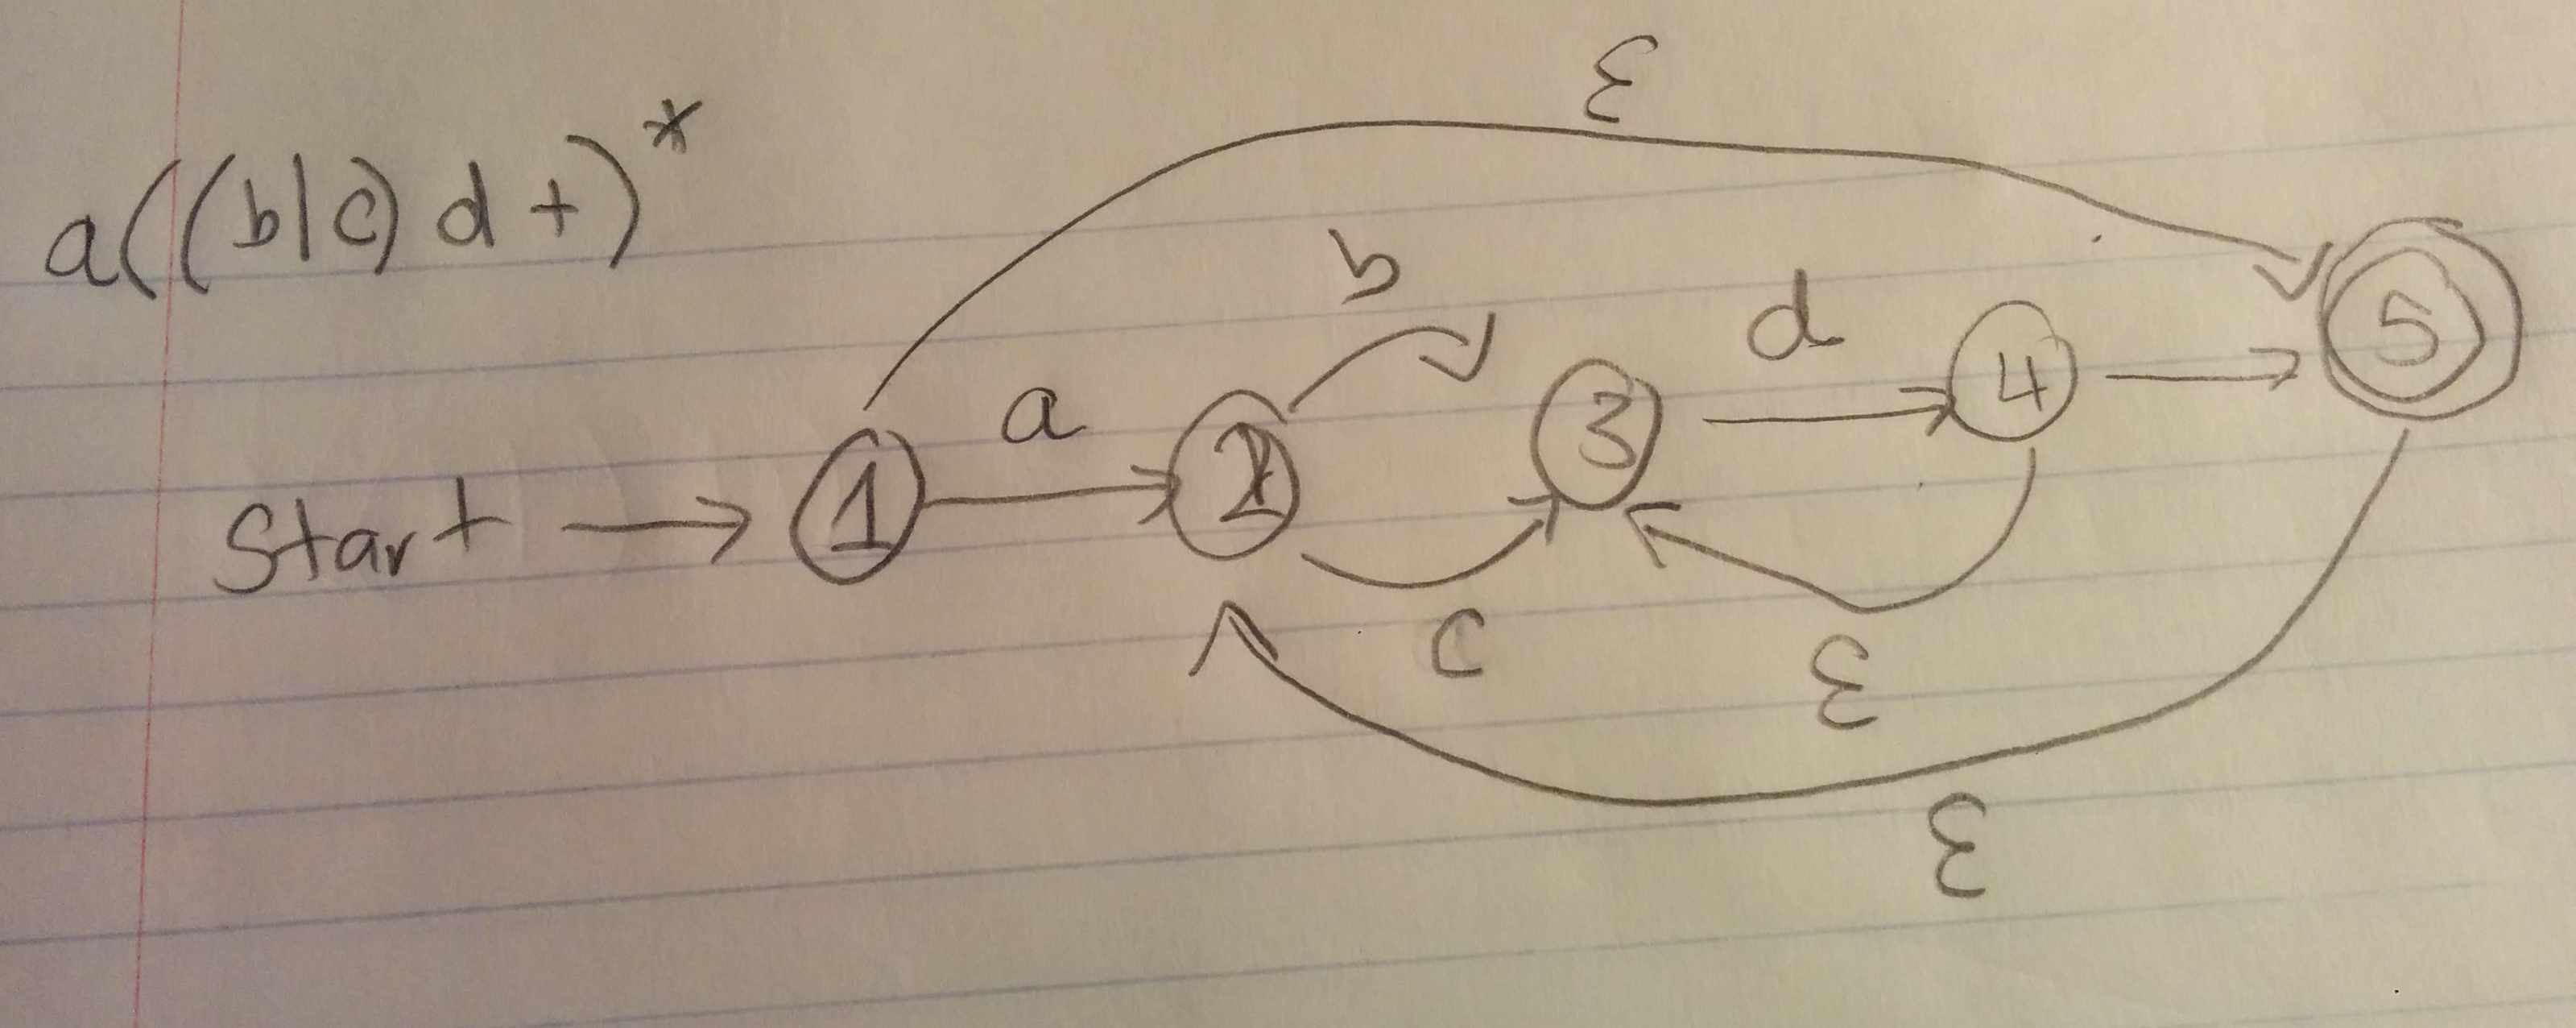
\includegraphics[scale=0.125]{hw21.png}

\subsection{Question 2.2}
\par Describe informally the kind of strings that is accepted by this NFA, and show a DFA that accepts the same language.
\par \includegraphics[scale=0.15]{hw22.png}

\subsection{Question 2.3}
\par Describe informally the kind of strings that is accepted by this DFA, and show a regular expression that accepts the same language.
\par A type of phrase that would fit here would be: `cbc', `cacba'
\par c (0 or more) then b, a or c (0 or more) OR a or b then a or c (0 or more) then b then a or b or c (0 or more)
\par This ends on both 1 or 2. So we have to take this into account
\par regular expression: c*(b(a$|$c)* $|$ (a$|$b(a$|$c)*b (a$|$b$|$c)*))

\section{Regular Expressions}
\par Running { celsius := 20; fahrenheit := celsius * 1.8 + 32; } on hacs gives:
\par LDF T ,  \#20
\par STF celsius , T  
\par LDF T\_1 ,  celsius    
\par LDF T\_2 ,  \#1.8    
\par MULF  T\_1\_31   ,  T\_1   ,  T\_2    
\par LDF T\_2\_88 ,  \#32    
\par ADDF  T\_82   ,  T\_1\_31   ,  T\_2\_88    
\par STF fahrenheit , T\_82

\end{document}  
